\documentclass{article}
\usepackage{url}
\usepackage{color}
\usepackage{pdfcolmk}
\usepackage{Sweave}
\begin{document}
\Sconcordance{concordance:hw1_report.tex:hw1_report.Rnw:%
1 4 1 1 0 53 1 1 2 1 0 5 1 12 0 1 2 1 1 1 2 1 0 3 1 12 0 1 2 1 1 1 2 1 %
0 1 1 6 0 1 1 12 0 1 2 2 1 1 2 6 0 1 1 5 0 1 1 7 0 1 1 8 0 1 2 2 1 1 2 %
20 0 1 2 30 1}

\DefineVerbatimEnvironment{Sinput}{Verbatim}{formatcom = {\color[rgb]{0, 0, 0.56}}}
\DefineVerbatimEnvironment{Soutput}{Verbatim}{formatcom = {\color[rgb]{0.56, 0, 0}}}
\graphicspath{{/Users/jacquelineroudes/Documents/GTL_courses/Data_Visual_Analytics}}
\begin{titlepage}
\vspace*{\stretch{1}}

\begin{center}

\includegraphics[scale=0.4]{GT_logo.jpeg}
\end{center}
\vspace*{\stretch{1}}
\hrulefill
\begin{center}\bfseries\huge
   HW1 Report \\
    R Programming\\
    \hrulefill
\end{center}
\vspace*{1cm}
\begin{minipage}[t]{0.4\textwidth}
  \begin{flushleft} \large
    \emph{Subject : \\
    CSE 6242 Spring 2017 - OMS}\\
  \end{flushleft}
\end{minipage}
\begin{minipage}[t]{0.6\textwidth}
  \begin{flushright} \large
    \emph{Author :} \\
    Melisande Zonta Roudes \\
    GT account name : mzr3 \\
  \end{flushright}
\end{minipage}
\vspace*{\stretch{2}}
\begin{flushright}
       Le \today 
\end{flushright} 

\end{titlepage}

\section{Get Familiar with R}

  Matlab being one of my main programming language, R is quite reassuring thanks to some similarities concerning the syntax of mathematic tools or graphics ones. Indeed, R and Matlab are both mathematical languages. Moreover, Python has also some particular objects in common with R like lists. Many other possibilities make of R a really powerful tool for statistics and data analysis.

In addition of some syntax particularities, what strikes me most in the R programming language is the power of dataframes. 
 
Indeed, at first sight, this object has rows and columns as a matrix, however the big difference stands in the possibility to store various types of objects (mode character, mode numeric, mode logical...).
 
While this kind of storage can be seen in the list which is is a special vector with elements of different modes including lists themselves, the list's content is not represented as an array. 
 
The distinguishing feature between a dataframe and a list is the constraint in the first of having a similar length of elements which explains the organisation in columns. 

So let's take an example of a ranking between countries which is a particularly convenient for dataframe. R has its own dataframes (mtcars, iris, diamonds) we used during these first lessons but we will elaborate one on our own. Datas were extracted from this document : \url{http://www.clesdusocial.com/IMG/pdf/europe-sociale-chiffres-classements.pdf}. This dataset analysis could show a link between the GDP of countries and Life Expectancy or between GDP and employment. Visualization would then play its role to make this induction.
To create our data-frame, we must gather the elements of each category in a list and then call the R function data.frame().

\begin{Schunk}
\begin{Sinput}
> Countries <- c("France","Germany","England","Italy","Luxembourg","Netherlands")
> GDP <- c(27.0,29.0,29.4,25.3,64.1,33.9)
> Employment <- c(65.2,70,71.5,58.7,90.0,77.2)
> Life.Expectancy.men <- c(77.5,77.4,77.3,78.5,76.7,78.1)
> ranking <- data.frame(Countries,GDP,Employment,Life.Expectancy.men)
> print(ranking)
\end{Sinput}
\begin{Soutput}
    Countries  GDP Employment Life.Expectancy.men
1      France 27.0       65.2                77.5
2     Germany 29.0       70.0                77.4
3     England 29.4       71.5                77.3
4       Italy 25.3       58.7                78.5
5  Luxembourg 64.1       90.0                76.7
6 Netherlands 33.9       77.2                78.1
\end{Soutput}
\end{Schunk}

We can build another one on the same pattern. The datas chosen gather only two modes : numeric and character, but we could have added in an other dimension some logical elements.
\begin{Schunk}
\begin{Sinput}
> Countries <- c("France","Germany","England","Italy","Luxembourg","Netherlands")
> Life.Expectancy.women <- c(84.5,82.7,81.7,84.2,82.2,82.5)
> ranking2 <- data.frame(Countries,Life.Expectancy.women)
> print(ranking2)
\end{Sinput}
\begin{Soutput}
    Countries Life.Expectancy.women
1      France                  84.5
2     Germany                  82.7
3     England                  81.7
4       Italy                  84.2
5  Luxembourg                  82.2
6 Netherlands                  82.5
\end{Soutput}
\end{Schunk}

One powerful function in R is the possibility of merging two data-frames horizontally with the merge() function. The example below merges ranking and ranking2 by all its key variables. It allows to add colums to our datasets as we can observe by calling the names() function.
\begin{Schunk}
\begin{Sinput}
> ranking_global <- merge(ranking,ranking2)
> names(ranking_global)
\end{Sinput}
\begin{Soutput}
[1] "Countries"             "GDP"                   "Employment"           
[4] "Life.Expectancy.men"   "Life.Expectancy.women"
\end{Soutput}
\begin{Sinput}
> print(ranking_global)
\end{Sinput}
\begin{Soutput}
    Countries  GDP Employment Life.Expectancy.men Life.Expectancy.women
1     England 29.4       71.5                77.3                  81.7
2      France 27.0       65.2                77.5                  84.5
3     Germany 29.0       70.0                77.4                  82.7
4       Italy 25.3       58.7                78.5                  84.2
5  Luxembourg 64.1       90.0                76.7                  82.2
6 Netherlands 33.9       77.2                78.1                  82.5
\end{Soutput}
\end{Schunk}

There are different ways of accessing the array's values as we saw in Chapter 7. We can obtain a column with the symbol $\$$ followed by name of the category we want. By specifying the location of the cell as in a matrix, we can have its value. The function head() allows us to access to a selected number of rows. Last but not least, we can create subset among our dataframes by applying a condition on values which is really useful to filter our datas according to some caracteristics.

\begin{Schunk}
\begin{Sinput}
> ranking_global$GDP
\end{Sinput}
\begin{Soutput}
[1] 29.4 27.0 29.0 25.3 64.1 33.9
\end{Soutput}
\begin{Sinput}
> ranking_global[1,2]
\end{Sinput}
\begin{Soutput}
[1] 29.4
\end{Soutput}
\begin{Sinput}
> head(ranking_global,2)
\end{Sinput}
\begin{Soutput}
  Countries  GDP Employment Life.Expectancy.men Life.Expectancy.women
1   England 29.4       71.5                77.3                  81.7
2    France 27.0       65.2                77.5                  84.5
\end{Soutput}
\begin{Sinput}
> subset(ranking_global,ranking_global$GDP > 30)
\end{Sinput}
\begin{Soutput}
    Countries  GDP Employment Life.Expectancy.men Life.Expectancy.women
5  Luxembourg 64.1       90.0                76.7                  82.2
6 Netherlands 33.9       77.2                78.1                  82.5
\end{Soutput}
\end{Schunk}

Finally, it would be a shame not to speak of the summary() function, which is in my mind the first call we should make to analyse a dataset. It provides an overview of the rows' and columns' names and above all indications on the values of these key variables (mean, max, min, median). It is really useful to detect outliers by comparing it with the mean.

\begin{Schunk}
\begin{Sinput}
> summary(ranking_global)
\end{Sinput}
\begin{Soutput}
       Countries      GDP          Employment    Life.Expectancy.men
 England    :1   Min.   :25.30   Min.   :58.70   Min.   :76.70      
 France     :1   1st Qu.:27.50   1st Qu.:66.40   1st Qu.:77.33      
 Germany    :1   Median :29.20   Median :70.75   Median :77.45      
 Italy      :1   Mean   :34.78   Mean   :72.10   Mean   :77.58      
 Luxembourg :1   3rd Qu.:32.77   3rd Qu.:75.78   3rd Qu.:77.95      
 Netherlands:1   Max.   :64.10   Max.   :90.00   Max.   :78.50      
 Life.Expectancy.women
 Min.   :81.70        
 1st Qu.:82.28        
 Median :82.60        
 Mean   :82.97        
 3rd Qu.:83.83        
 Max.   :84.50        
\end{Soutput}
\end{Schunk}

\section{Log Gamma (Loop)}

\section{Log Gamma (Recursive)}

\section{Sum of Log Gamma}

\section{Compare Results to Built-in R Function}

After having implemented different methods for the sum of Log Gamma, it's time to compare their efficiency regarding running time. To have an element of reference, we will compute the sum of Log Gamma with the Built-in function lgamma(). This function has been implemented in hw1.r file. We use the system.time() function and store the first element which is the user time.

\begin{figure}[!h]
\centering
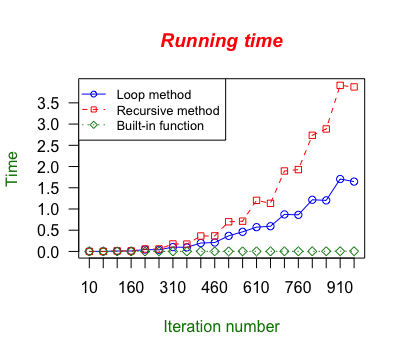
\includegraphics[width=.8\textwidth]{Time_100_iterations.png}
 \caption{Comparison between the 3 function over 1000 iterations}
\label{courbe1}
\end{figure}

We can observe on figure~\ref{courbe1} that recursive method consumes three times more than loop method. However, loop method itself is far less computing time efficient than the R built-in function.

\begin{figure}[h!]
\centering
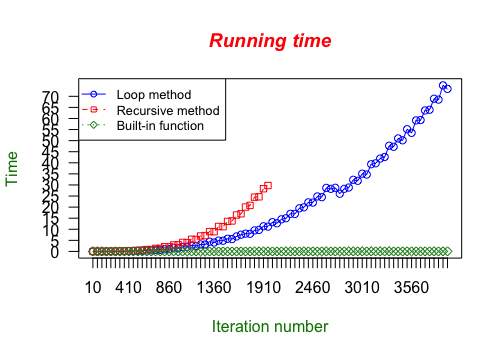
\includegraphics[width=.9\textwidth]{time_4000_iteration.png}
 \caption{Comparison between the 3 function over 4000 iterations}
\label{courbe2}
\end{figure}

To test those 3 functions, we will compute Loop method and Built-in function over 4000 iterations and only over 2000 iterations for recursive method to avoid overflow.
On figure~\ref{courbe2}, we can see again the same ratio (1 to 2) between the two implemented methods. Concerning the computing time reached at 4000 iterations, the difference between the Built-in function and the loop method is striking. Hence, we should rather compute the sum of Log Gamma with the R built in function when n becomes bigger.

\end{document}
